\definecolor{CodeColor}{HTML}{1f77b4}       
\definecolor{TruthTableColor}{HTML}{2ca02c} 
\definecolor{NLCoTColor}{HTML}{ff7f0e}      
\pgfplotsset{compat=1.18}
\begin{figure*}[t]
\centering
\vspace{-2em}
\begin{tikzpicture}
%%% ------------ 图1：Dot Plot + Trend Line + Note ------------
\node[anchor=south west] (a) at (0,0) {
\begin{tikzpicture}
\begin{axis}[
    width=0.33\textwidth,
    height=4.3cm,
    axis background/.style={fill=gray!10},
    xlabel={\small \makecell{\# Benchmark\\ (a) Uniqueness Ratio}},
    ylabel={\small Solve Rate (\%)},
    symbolic x coords={FOLIO, ProofWriter},
    xtick=data,
    ybar stacked,
    bar width=17pt,
    ymajorgrids=true,
    grid style={dashed,gray!30},
    enlarge x limits=0.5,
    tick align=inside,
    clip=false,
    ymin=0, ymax=40,
    tick label style={font=\small},
    label style={font=\small},
    x tick label style={align=center, yshift=-0.3ex},
    axis lines=box,
    legend style={
        at={(0.02,0.99)}, anchor=north west,
        font=\tiny,
        fill=white, fill opacity=0.7,
        draw=black!40,
        fill=gray!10,
        legend columns=1
    },
    legend image code/.code={
      \draw[draw=none, fill=#1] (0cm,-0.1cm) rectangle (0.4cm,0.1cm);
    }
]
\addplot+[fill=CodeColor, draw=none] coordinates {
    (FOLIO,2.46) (ProofWriter,6.67)};
\addplot+[fill=TruthTableColor, draw=none] coordinates {
    (FOLIO,5.41) (ProofWriter,11.0)};
\addplot+[fill=NLCoTColor, draw=none] coordinates {
    (FOLIO,8.87) (ProofWriter,18.2)};
\legend{Code, Truth Table, NL CoT}
\end{axis}
\end{tikzpicture}
};

%%% ------------ 图2：Sampling Diversity ------------
\node[anchor=south west] (b) at (0.31\textwidth,0) {
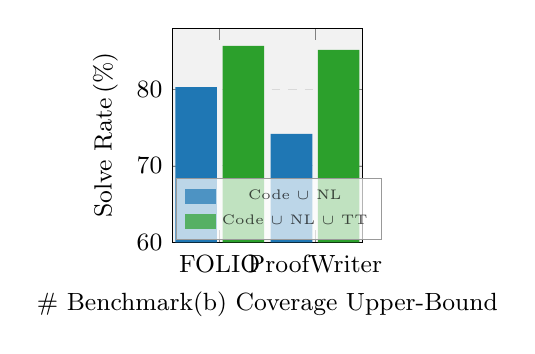
\begin{tikzpicture}
\begin{axis}[
    width=0.33\textwidth,
    height=4.3cm,
    axis background/.style={fill=gray!10},
    xlabel={\small \makecell{\# Benchmark\\(b) Coverage Upper-Bound}},
    ylabel={\small Solve Rate\,(\%)},
    symbolic x coords={FOLIO,ProofWriter},
    xtick=data,
    ybar,
    bar width=15pt,
    ymajorgrids=true,
    grid style={dashed,gray!30},
    enlarge x limits=0.5,
    tick align=inside,
    clip=false,
    ymin=60, ymax=88,
    tick label style={font=\small},
    label style={font=\small},
    axis lines=box,
    x tick label style={align=center, yshift=-0.3ex},
    legend style={
      at={(0.02,0.30)}, anchor=north west,
      font=\tiny,
      fill=white, fill opacity=0.7,
      draw=black!40,
      legend columns=1
    },
    legend image code/.code={
      \draw[draw=none, fill=#1] (0cm,-0.1cm) rectangle (0.4cm,0.1cm);
    }
]
\addplot+[fill=CodeColor, draw=none] coordinates {
    (FOLIO,80.3) (ProofWriter,74.17)};
\addplot+[fill=TruthTableColor, draw=none] coordinates {
    (FOLIO,85.7) (ProofWriter,85.17)};
\legend{Code $\cup$ NL, Code $\cup$ NL $\cup$ TT}
\end{axis}
\end{tikzpicture}
};

%%% ------------ 图3：无边框美化版堆叠柱状图 ------------
\node[anchor=south west] () at (0.62\textwidth,0) {
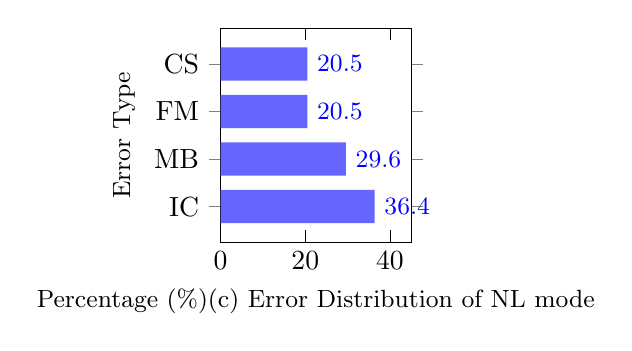
\begin{tikzpicture}
  \begin{axis}[
    xbar,
    bar width=12pt,
    width=0.33\textwidth,
    height=4.3cm,
    xmin=0, xmax=45,
    xlabel={\small \makecell{Percentage (\%)\\(c) Error Distribution of NL mode }},
    symbolic y coords={
      IC,
      MB,
      FM,
      CS
    },
    ytick=data,
    ylabel={\small Error Type},
    nodes near coords,
    every node near coord/.append style={
      font=\small,
      xshift=0pt
    },
    axis lines=box,
    major x grid style={dashed,gray!30},
    major x tick style={black},
    enlarge y limits=0.25
  ]
    % Our finetune
    % \addplot+[draw=none, fill=blue!60] coordinates {
    %   (36.2,IC)
    %   (33.0,MB)
    %   (22.3,FM)
    %   (17.0,CS)
    % };
    % Baseline without finetune
    \addplot+[draw=none, fill=blue!60] coordinates {
      (36.4,IC)
      (29.6,MB)
      (20.5,FM)
      (20.5,CS)
    };
  \end{axis}
\end{tikzpicture}
};

\end{tikzpicture}

\vspace{-1em}
% \caption{(a) Percentage of examples solved exclusively by each thought paradigm using Qwen-2.5-7B-Instruct: roughly 20\% on FOLIO and 35\% on ProofWriter. (b) Upper-bound coverage when combining paradigms: the trio of code + natural language (NL) + truth table outperforms code + NL~\cite{Xiong2024HYBRIDMINDMS}. (c) Error types of widely used natural language modes: invalid-converse and missing-branch errors together make up nearly 70\% of all failures. CS: commonsense injection; FM: factual misquote; MB: missing‑branch; IC: invalid‑converse. }
\caption{\footnotesize{(a) Qwen‑2.5‑7B‑Instruct solves $\simeq$20\% of FOLIO and $\simeq$35\% of ProofWriter exclusively per paradigm. (b) Code+NL+truth‑table yields higher upper‑bound coverage than code+NL alone~\cite{Xiong2024HYBRIDMINDMS}. (c) In NL modes, invalid‑converse (IC) and missing‑branch (MB) errors comprise $\simeq$66\% of failures (CS: commonsense injection; FM: factual misquote). Percentages sum to more than 100\% because some cases exhibit multiple error types. We provide illustrative examples in Appendix \ref{subsec:example_error_types}}}
\label{fig:motivation}
\vspace{-2em}
\end{figure*}
